\section{Introduction}

Cartons have been widely used in the packaging industry to organize, ship and deliver various commodities including food, daily necessities and electronic components. Instead of the very basic packaging shapes like cuboids, there exist multiple fantastic cartons to package wedding candies or wine bottles. 
These various designs increase much popularity, not to mention they are environmental friendly due to their recycling and degradability~\cite{Mullineux:2010:CSC:1739328.1739673}.

Cartons are usually designed based on experience and trial-and-error.
\reply{Designers often start package design by generating 2D vector artwork, then a 3D mockup is essential to be made for designers and clients to see the real appearance. There are two ways to create a 3D mockup, a digital mockup is a great way of showing how the design would appear with lower cost, and a practical mockup can be helpful when making sure the size is correct and making final decision.}

In recent years, there are software packages developed help designers improve efficiency and productivity.
%For example, KASEMAKE~\cite{KASEMAKE} can help users edit existing structural designs from a database by feed in the required size and materials.
\reply{For example, a plug-in for adobe illustrator named STUDIO~\cite{STUDIO} can generate 3D models by manually assigning angles to folding edges, and with the model, users can turn their ideas into beautiful 3D images.}
\reply{However, the existing softwares still need a lot manual work to design packages.
%Researchers have also studied in obtaining 2D layouts from unfolding 3D objects for decades. However, the unfolded layouts are fragile in some parts which are not suitable for fabrication~\cite{Tai2004Unfolding} and sometimes are not feasible to fold.
In order to create a virtual 3D model and explore layouts' diversity,} our idea is to fold the existing layout directly into 3D model, and by manipulating the corresponding model to reach a diverse layout.

However, based on given planar layout of a carton only, it is nontrivial to formulate the problem of 3D model construction mathematically, because the information extracted from the 2D layout such as edge length and vertex degree may cause ambiguities on account of repeated edges and vertexes. Moreover, Biedl et al.~\cite{Biedl:2005:NFP:1090462.1646553} proved that given a polygon and a set of creases, it is NP-hard to know whether a polyhedron can be obtained by folding along the creases, which can also illustrate the difficulty of our problem in some way.

\begin{figure}
	\centering
	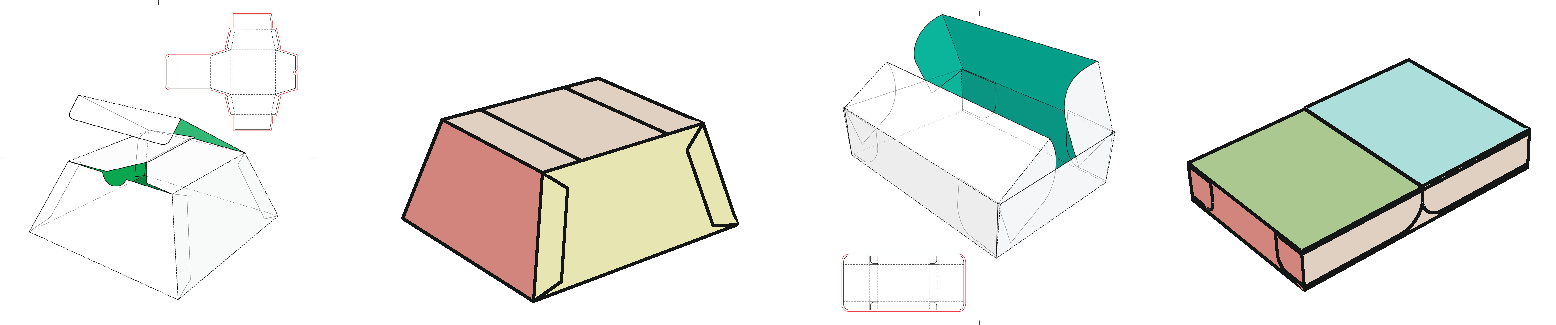
\includegraphics[width=0.9\textwidth]{images/artist}
	\caption{Two cartons and their layouts designed by artist, and the corresponding model folded by our system.}
	\label{fig:artist}
\end{figure}

%pick existing structural designs from a database and feed in the required size and materials. Moreover, users can re-import a finished artwork to show the print on the structural designs and fold it into a three-dimensional view in seconds.



%Papercraft problems have attracted a large mount of attentions in computer graphics community for decades.
%Researchers primarily concerned with the following issues: (1) computational algorithm and mathematic analysis for folding origami~\cite{Ida:2007:MOC:1802954.1803021,Lang:1996:CAO:237218.237249,xl-idetc-14}; (2) problems on the folding polygon and unfolding polyhedron~\cite{Bern:2003:UPC:636968.636970,O'Rourke:1998:FUC:646319.686376,Rourke2008Unfolding}, and some proofs to show the problem complexity of folding to polyhedron~\cite{Biedl:2005:NFP:1090462.1646553,Biedl2004When,Lubiw1996When}; (3) other specific structure folding problems like Kinetogami which comprises multi-primitive and reconfigurable units folded from a single sheet of paper~\cite{Gao2013Kinetogami} and applications to show the folding behavior of paper~\cite{Thiel1998,Kishi:1998:OFP:786112.786279,Nimnual2007Virtual,Shimanuki2009Construction}. 
%
%Although previous techniques solved a number of problems in paper folding, they have not considered intelligent construction 3D models given 2D paper layouts. 
%In this paper, we focus on the carton folding problem and introduce an interactive shape optimization method.
 
 
In order to solve the folding cartons just from 2D layouts, we solve a optimization problem given on  set of shape constraints.
Moreover, an interactive design and exploration framework is developed to allow users to visualize the planar layouts and the corresponding model in a 3D view, and edit the 3D model freely. Figure~\ref{fig:artist} shows our folding results based on the layouts designed by artists. 

The contribution of this paper includes the following:

(1) An interactive and explorative system to manipulate the shape of 3D carton: It creates the corresponding 3D realization by initialization and user interaction, and users are allowed to edit the 3D model to explore deformed layouts automatically.

(2) A collection of shape constraints represented through a set of points to implement shape optimization: Observed from existing cartons, constraints are summarized including face rigidity and coplanarity to keep the shape of cartons. Besides, computer-aid detection like vertex merging and face pasting are brought to give users suggestions. 